\chapter{Internet věcí}
\label{ChapterInternetVeci}

Cílem Internetu věcí (IoT - Internet of Things) je propojení zařízení, systémů a~služeb za účelem poskytnutí více dat, která mohou být převedena na informace a~informace potom na znalosti, které mohou být následně aplikovány. Princip IoT je tedy sběr dat, ty jsou následně uložena a analyzována a poté dojde ke~sdílení výsledků. V rámci IoT se vytvořily dva hlavní směry, průmyslový Internet věcí (iIoT - Industry IoT) a spotřebitelský Internet věcí (cIoT - Customer IoT) \cite{iot_svet_hardware_internet_veci, iot_pohanka_internet_veci}. Rozdíly obou směrů jsou shrnuty v Tab.~\ref{TableIOT}.

\section{Spotřebitelský Internet věcí}
Spotřebitelský Internet věcí se zaměřuje na spotřebitelská zařízení, IT a telekomunikační zařízení a další. Jsou zde využívána zařízení zjednodušující každodenní život pomocí automatizace v domácnosti, chytrých zařízení nebo pomocí nositelné elektroniky. Hlavní výhodou je zvýšení uživatelského zážitku (QoE - Quality of Experience).

\section{Průmyslový Internet věcí}
Průmyslový Internet věcí vychází z M2M (Machine to Machine) a rozšiřuje komunikaci o možnost uložení, analýzy a zobrazení dat. Jedná se o IoT zařízení a systémy, které jsou používány v průmyslových odvětvích, jako jsou průmyslová automatizace, energetický průmysl a zdravotnictví. Hlavním zaměřením je efektivnější využívání zdrojů, snížení provozních nákladů, zvýšení efektivity či bezpečnosti. V praxi může sloužit například pro zajištění bezpečnosti pracovníků či automatizaci údržby. 


\begin{table}[!ht]
\caption{Porovnání průmyslového a spotřebitelského IoT \cite{iot_svet_hardware_internet_veci, iot_pohanka_internet_veci}}
\vspace{-10pt}
\label{TableIOT}
\begin{center}
\small
\begin{tabular}{|c|c|c|}
\hline
 & \textbf{Spotřebitelský IoT} &  \textbf{Průmyslový IoT} \\ \hline \hline
\textbf{Zaměření} & Spotřebitel. & Průmysl. \\ \hline
\textbf{Zařízení} & \begin{tabular}[c]{@{}c@{}}Chytré zařízení\\ a nositelná elektronika.\end{tabular} & \begin{tabular}[c]{@{}c@{}}Stroje, zařízení\\  a průmyslová automatizace.\end{tabular} \\ \hline
\textbf{Důležitost} & \begin{tabular}[c]{@{}c@{}}Nejedná se o životně \\ důležité systémy.\end{tabular} & \begin{tabular}[c]{@{}c@{}}Jedná se o životně\\ důležité systémy.\end{tabular} \\ \hline
\textbf{Využití} & \begin{tabular}[c]{@{}c@{}}Zvýšení uživatelského\\ zážitku.\end{tabular} & \begin{tabular}[c]{@{}c@{}}Lepší využívání zdrojů, \\  snížení provozních nákladů, \\ zvýšení efektivity či bezpečnosti.\end{tabular} \\ \hline \hline
\end{tabular}
\vspace{-10pt}
  \end{center}
\end{table}

\subsection{Průmysl 4.0}

Současný trend digitalizace a s ní související automatizace výroby je označován jako Průmysl 4.0. Koncept vychází z dokumentu, který byl představen na veletrhu v~Hannoveru v roce 2013. Předpokládá se, že v horizontu následujících 10 až 15 let nastane příchod čtvrté průmyslové revoluce, která přinese radikální změnu ve srovnání s nynějším výrobním procesem. Podle této myšlenky vzniknou chytré továrny, které budou využívat kyberneticko-fyzikální systémy. Ty převezmou opakující se~a~jednoduché činnosti, které do té doby vykonávali lidé. Má zahrnovat kompletní (viz Obr.~\ref{SchemaPrumysl4}) digitalizaci, robotizaci a automatizaci většiny současných lidských činností pro zajištění větší rychlosti a efektivity výroby přesnějších, osobitějších, spolehlivějších a levnějších produktů, současně pro efektivnější využití materiálů a ekologičtější průmysl i lidský život \cite{uvod_prumysl_4_pdf}.


	\begin{figure}[!ht]
  \begin{center}
   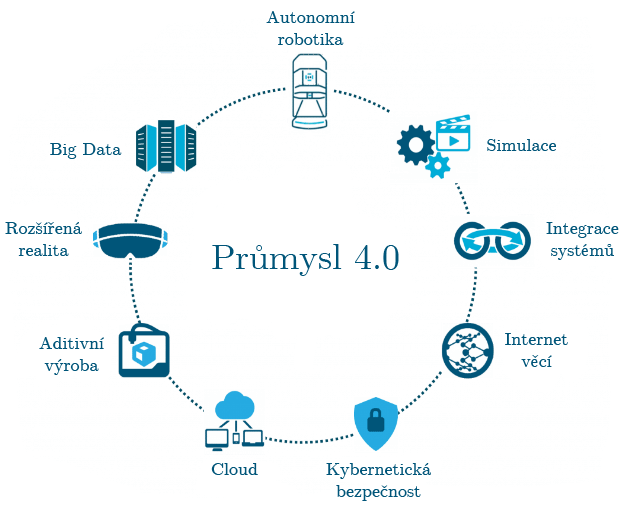
\includegraphics[scale=0.45]{obrazky/iot_industry4}
  \end{center}
	\vspace{-20pt}	
  \caption{Schéma odvětví Průmyslu 4.0}
	\label{SchemaPrumysl4}
\vspace{-10pt}	
\end{figure}



Na průmyslové úrovni má jít o nahrazení manuální lidské práce robotizací, současné manuální zadávání výrobních dat a postupů má být nahrazeno automatickým elektronickým předáváním informací mezi jednotlivými výrobními komponentami a~materiálmi. Významné změny mají i ve spojistosti s automatizovaným průmyslem nastat v oblasti domácností a běžného bydlení, kde mají být jednotlivé domácí systémy vzájemně elektronicky propojeny a jejich vzájemná koordinovaná spolupráce bude maximalizovat efektivitu a současně minimalizovat spotřebu médií.

V reflexi na tento trend v září 2015 vydalo Ministerstvo průmyslu a obchodu Národní iniciativu Průmysl 4.0~\cite{uvod_prumysl_4_pdf}, podle které bude revoluce příležitostí pro růst a~konkurenceschopnost českých firem a České republiky vůbec.









